%\documentclass[12pt,a4paper,prb,superscriptaddress,
% tightenlines,  % single-spaced
%]{revtex4}
\documentclass[12pt,prb,aps]{revtex4}
\usepackage{amsmath,amssymb,physics}
\usepackage{graphicx} % For figures with images
\usepackage{natbib} % bibliography
% \setcitestyle{super, sort&compress, comma} % chemistry style (prb's default)
\usepackage{hyperref} % Clickable links in the document and their colors
\hypersetup{
    colorlinks=true, % false: boxed links; true: colored links
    linkcolor=cyan, % color of internal links
    citecolor=magenta, % color of links to bibliography
    filecolor=magenta, % color of file links
    urlcolor=cyan, % color of external links
    runcolor=cyan
}

\begin{document}

\title{Vibronic Coupling Effects in the Photoelectron Spectrum of Ozone: A
Coupled-Cluster Approach}

\author{Pawe{\l} W{\'o}jcik$^a$,  Hanna Reisler$^a$, P{\'e}ter G. Szalay$^b$, Anna I. Krylov$^{a,\dagger}$, John F. Stanton$^{b,c,*}$\\
{\small $^a$ Department of Chemistry, University of Southern California, Los Angeles, California 90089, USA}\\
{\small $^b$  Laboratory of Theoretical Chemistry, Institute of Chemistry, ELTE
E{\"o}tv{\"o}s Lor{\'a}nd University, P{\'a}zm{\'a}ny P{\'e}ter stny. 1/A,
Budapest, Hungary}\\
{\small $^c$ Quantum Theory Project, Departments of Chemistry and Physics, University of Florida, Gainesville, FL, USA 32611}\\
{$\dagger$ krylov@usc.edu; $^*$ jfstanton137@gmail.com}}


\date{\today}

\begin{abstract}
One of the most important areas of application for equation-of-motion coupled
cluster (EOM-CC) theory is the prediction, simulation, and analysis of
various types of electronic spectra. 
In this work, the EOM-CC method for ionized states, known
as EOM-IP-CC, is applied to the closely lying and coupled pair of states of the
ozone cation --- ${\tilde X}^2$A$_1$ and ${\tilde A}^2$B$_2$ --- using highly accurate 
treatments including up to the full single, double, triple, and quadruple excitations
(EOM-IP-CCSDTQ). Combined with a venerable and powerful method for
calculating vibronic spectra from the Hamiltonian produced by EOM-IP-CC
calculations, the simulations yield a spectrum that is in good agreement with
the photoelectron spectrum of ozone. Importantly,  the
calculations suggest that the adiabatic gap separating these two electronic
states is somewhat smaller than currently thought; an assignment of the
simulated spectrum together with the more precise band positions of the
experimental measurements suggests that this energy gap is 1,366$\pm$65
cm$^{-1}$.
\end{abstract}

\maketitle

\section{Introduction}

Amongst the brotherhood of triatomic molecules, it cannot be denied that water
(H$_2$O) is the most important, the most highly studied, and the most
well-understood. Beyond H$_2$O, many triatomic molecules that have
an environmental, technological or biological importance have been subjected
to many studies and are understood to various levels of detail. Perhaps the
most interesting such case is ozone (O$_3$), which has a vast number of
important properties, a very rich history of study \cite{chappuis}, and 
unlike the relatively simple water molecule, a profound quantum-mechanical
complexity \cite{Babikov:anomalousOzone:2003}. Structurally, while
we think of ozone as having two distinct kinds of oxygen atoms (and an NMR experiment would reveal that), the full molecular Hamiltonian does not distinguish
between them. Rather, it yields the three equivalent structures separated by a
barrier that lies tantalizingly close to the O$_3$ $\rightarrow$ O$_2$ + O
dissociation threshold (102.4 kJ/mol) \cite{Ruscis:ATcT:2022}, as shown in 
Fig. \ref{fig:3fold}.
In reality, the
energy levels of ozone all have a near triple ($e+a$) degeneracy, albeit with
a tunneling splitting so small that it can be ignored, along with a
semi-infinite lifetime (despite opposing opinion
\cite{Boggs:BerryOzone:2006}). More than a half century ago, this intriguing
aspect of the ozone molecule was first discussed by Berry
\cite{Berry:Ozone:1960}.

\begin{figure}[h!]
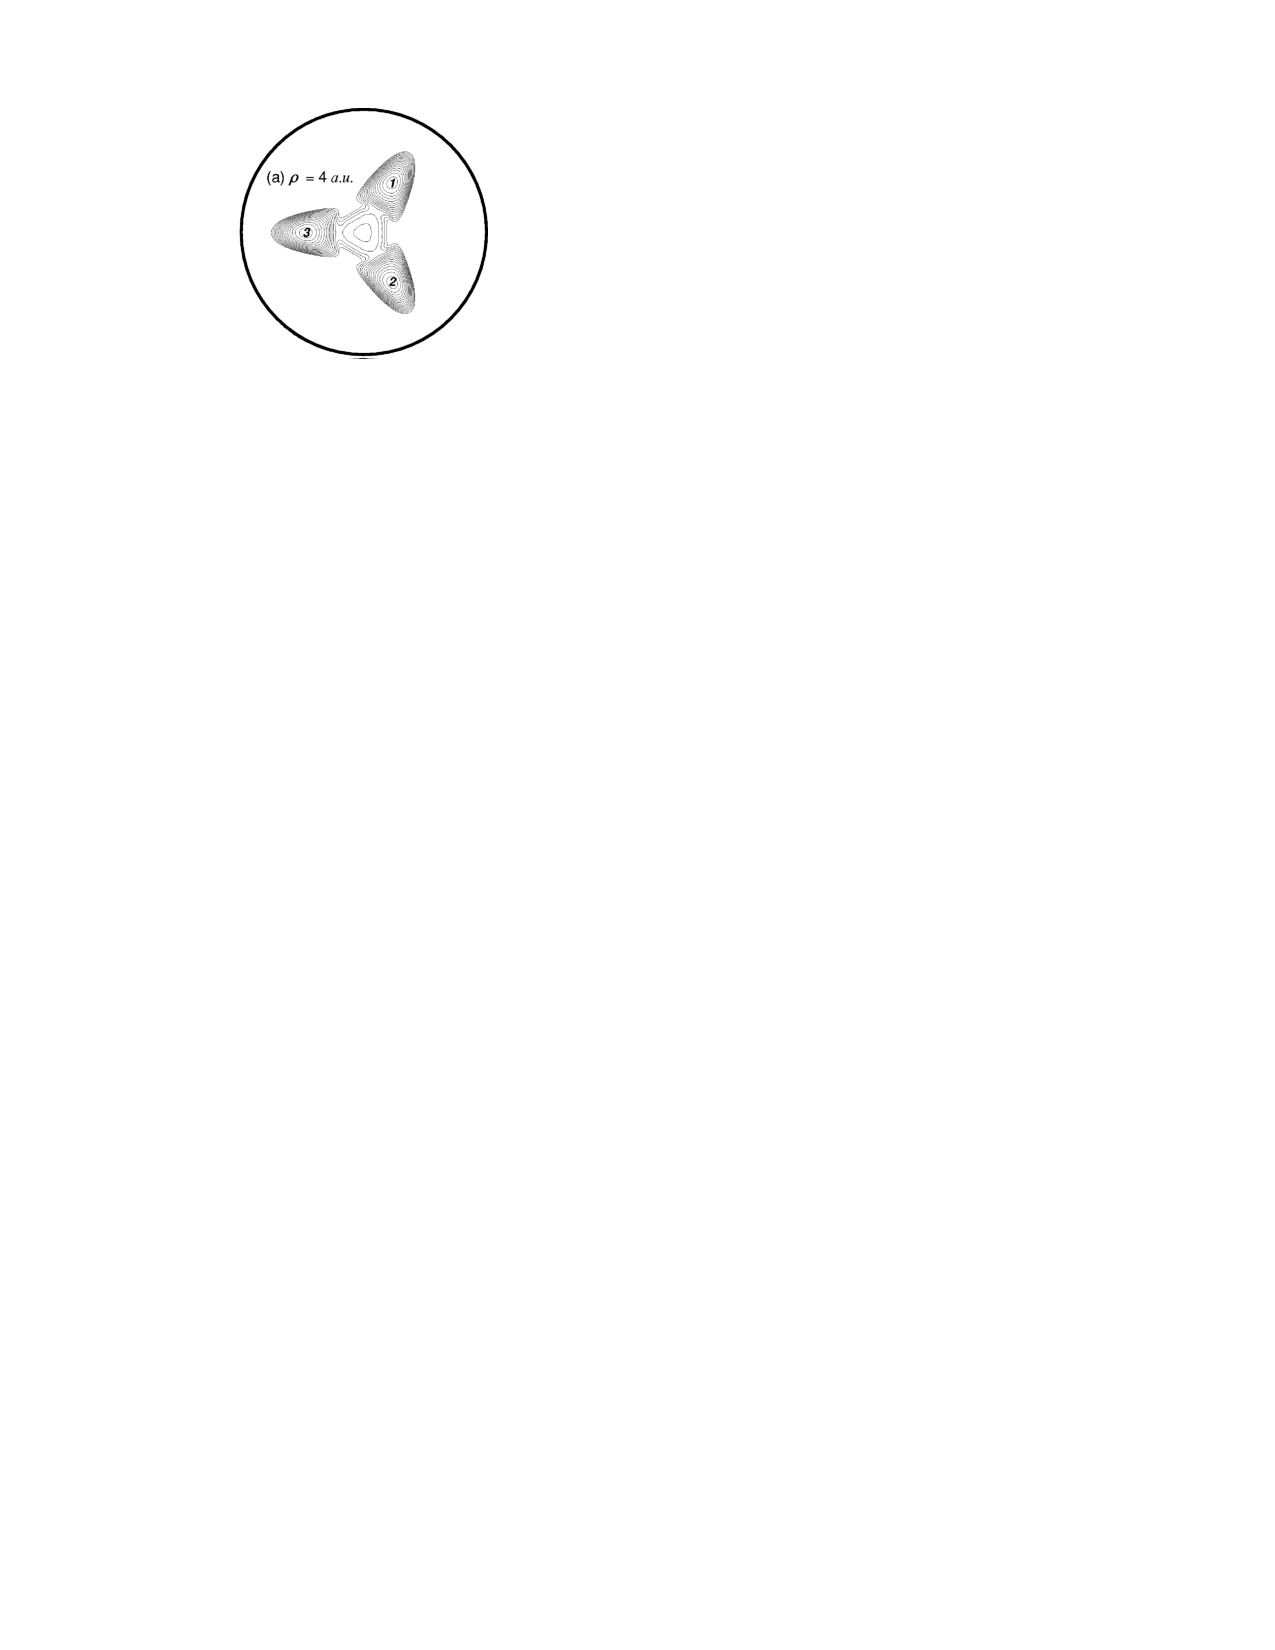
\includegraphics[width = 8 cm]{./figures/OzonePES3fold.pdf}
\caption{Two-dimensional slice of the potential energy surface of ozone in hyperspherical coordinates at the value of hyperradiuns $\rho$=4 a.u. (the lowest contour is at 1 eV below the dissociation limit). The slice shows three equivalent minima corresponding to 
C$_{2v}$ structures separated by large barriers. 
Reproduced with permission from Ref. \citenum{Babikov:Ozone:2003}.
    \label{fig:3fold}}
\end{figure}

Beyond the structural aspects of ozone, other mysteries surround this
curious molecule. For example, the distribution of the eighteen distinct
$^{16}$O/$^{17}$O/$^{18}$O isotopologues in the Earth's atmosphere differs
from what is expected based on the natural isotopic abundance, a puzzle that
has been open for more than three decades
\cite{Mauersberger:OzoneMystery:1990,Babikov:Ozone:2003}. 

Among quantum chemists, ozone has a notorious history, owing to its strong
diradical character causing significant difficulties in calculations of its
ostensibly simple ground-state molecular properties. An early 1989 study
\cite{Stanton:Ozone:1989, Stanton:Ozone:1989b} by the Bartlett group and
collaborators found that the CCSD+T(CCSD) method predicted that the molecular
equilibrium structure of ozone would have C$_s$ symmetry (that is, the
asymmetric stretching harmonic frequency computed by this method is
imaginary), a finding that led to a search for better treatment of
non-iterative triple excitations, ultimately leading to the well-known CCSD(T)
method \cite{Raghavachari:89, Urban:ccsd(t):1985, GenrefCCSD(T):93}. While
CCSD(T) and higher-level coupled-cluster methods available today
\cite{kucharski:ccsdtq:1992, Kallay:CCHigh, Matthews:ncc:2015} do a good job
in describing the equilibrium structure and vibrational potential, an elaborate multireference configuration interaction calculations can describe 
the entire ground-state surface out to the dissociation limit
\cite{Schinke:Ozone:2001,Babikov:Ozone:2003,Dawes:ozone:2013}, facilitating calculations of spectroscopy and chemical reactions of ozone.
As such, the quantum chemical understanding and
fidelity for the ground electronic state of O$_3$ is now at a mature level.

\begin{figure}[h!]
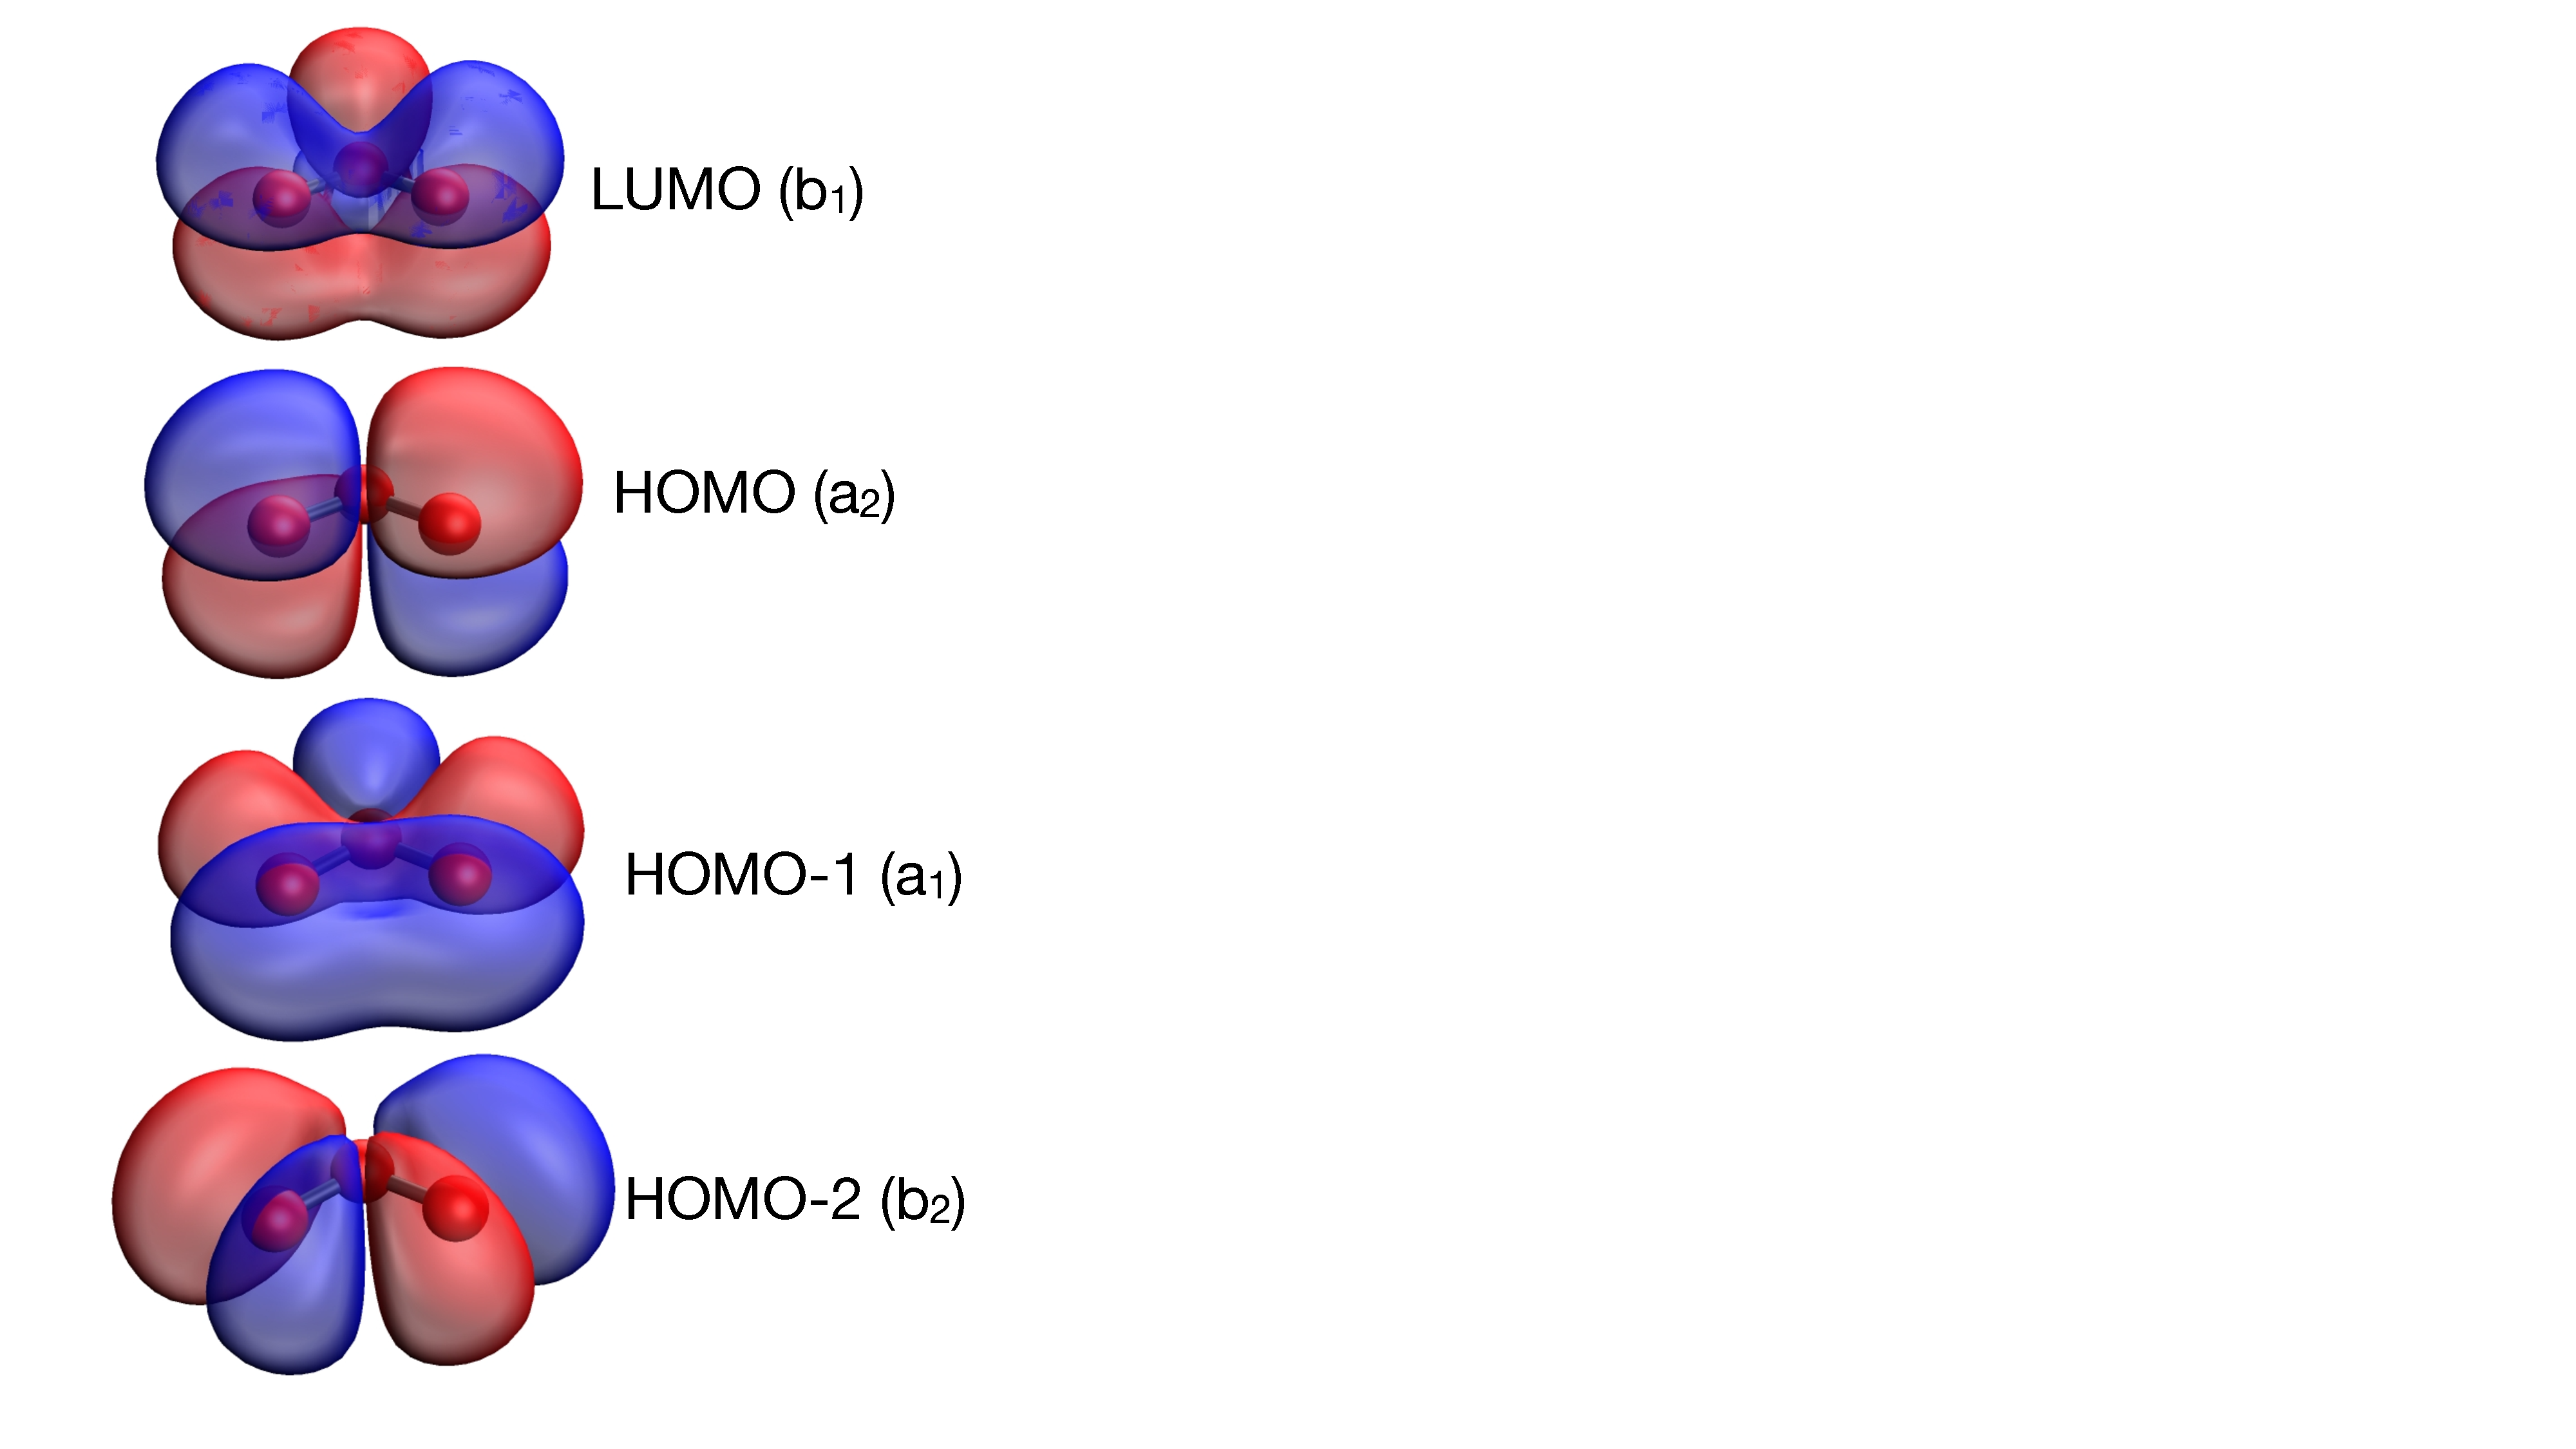
\includegraphics[width = 6cm]{./figures/MOs.pdf}
\caption{Frontier molecular orbitals of ozone; HF/6-31G*. The lowest states of the ozone 
cation are $^2$A$_1$ and $^2$B$_2$ derived by ionization from the HOMO-1 and HOMO-2, respectively.
    \label{fig:MOs}}
\end{figure}

Qualitatively, the challenge posed to electronic structure theory by ozone
ultimately arises from its closely spaced highest-occupied ($a_2$) and
lowest-unoccupied ($b_1$) molecular orbitals (HOMO and LUMO, respectively; see Fig. \ref{fig:MOs}), giving rise to the following wavefunction:
\begin{eqnarray}
X^1A_1 = C_1 [core]^6 (3a_1)^2 (2b_2)^2 (4a_1)^2  (5a_1)^2 (3b_2)^2  (1b_1)^2   (4b_2)^2 (6a_1)^2 (1a_2)^2 (2b_1)^0 + \\
C_2
[core]^6 (3a_1)^2 (2b_2)^2 (4a_1)^2  (5a_1)^2 (3b_2)^2  (1b_1)^2 (4b_2)^2 (6a_1)^2 (1a_2)^0
(2b_1)^2.
\end{eqnarray}
%The weights of these two leading configurations are $C_1\approx$0.952 and $C_2\approx$0.005, according to the EOM-SF-CCSD (EOM-CCSD with spin-flip) calculations\cite{sfccsd}.
%{\bf changing notations, need to check with John! This is confirmed by SF.}
The two electron configurations $[\cdots]a_2^2 b_1^0$ and $[\cdots]a_2^0 b_1^2$ 
%$[\cdots]b_2^2 a_1^0$ and $[\cdots]b_2^0 a_1^2$ 
mix strongly (the weights of these two leading configurations are $C_1\approx$0.952 and $C_2\approx$0.005,
according to the EOM-SF-CCSD (EOM-CCSD with spin-flip) calculations\cite{sfccsd}), 
posing the aforementioned challenges with (especially
single-reference) quantum-chemical methods.   
A second feature consequence of
the symmetry and energetic proximity of these two orbitals is that the ozone
cation (which is isoelectronic to the NO$_2$ radical) has closely lying
$^2$A$_1$ and $^2$B$_2$ electronic states derived by ionization from the HOMO-1 and HOMO-2, respectively (see Fig. \ref{fig:MOs}).
Like the associated states in NO$_2$,
these two states are plagued by orbital symmetry breaking
\cite{Davidson:SymmBreak:76}, a problem that greatly complicates
their quantum-chemical treatment.  One of the many
accomplishments of the Bartlett group has been the integral role played by
them in the development of equation-of-motion coupled-cluster theory
\cite{Stanton:93:EOMCC, Nooijen:EOMEA:95, Bartlett:CC_review:07} (EOM-CC, also
known as linear response coupled-cluster theory \cite{Koch:90:LinResp}). These
methods provide a very efficient and simple way to treat certain classes of electronic structure
that are often termed ``multireference problems" \cite{Krylov:EOMRev:07,Krylov:OSRev}, and
are ideally suited to studying reactive intermediates, radicals,
diradicals, and electronically excited states. From a somewhat wider
viewpoint, the existence of closely spaced electronic states always carries
the potential for (possibly strong) vibronic coupling, a phenomenon that can
play an important role in molecular dynamics and spectroscopy. 
Indeed, one of
the great successes of EOM-CC methods has been in their ability --- if and only
if combined with vibronic coupling models --- to enable high-quality
simulations of complicated electronic spectra.  Such work provides important
insights into the nature of vibronic coupling in molecular systems, as has been
exemplified by various application studies (for example, see
Refs.~\citenum{Stanton:NO3:07} and~\citenum{Koppel:02}). In the case of ozone cation, 
the two lowest electronic states separated by a small gap of $\sim$0.1 eV are coupled  
by the asymmetric stretch of b$_2$ symmetry (Fig. \ref{fig:vib}). 


\begin{figure}[h!]
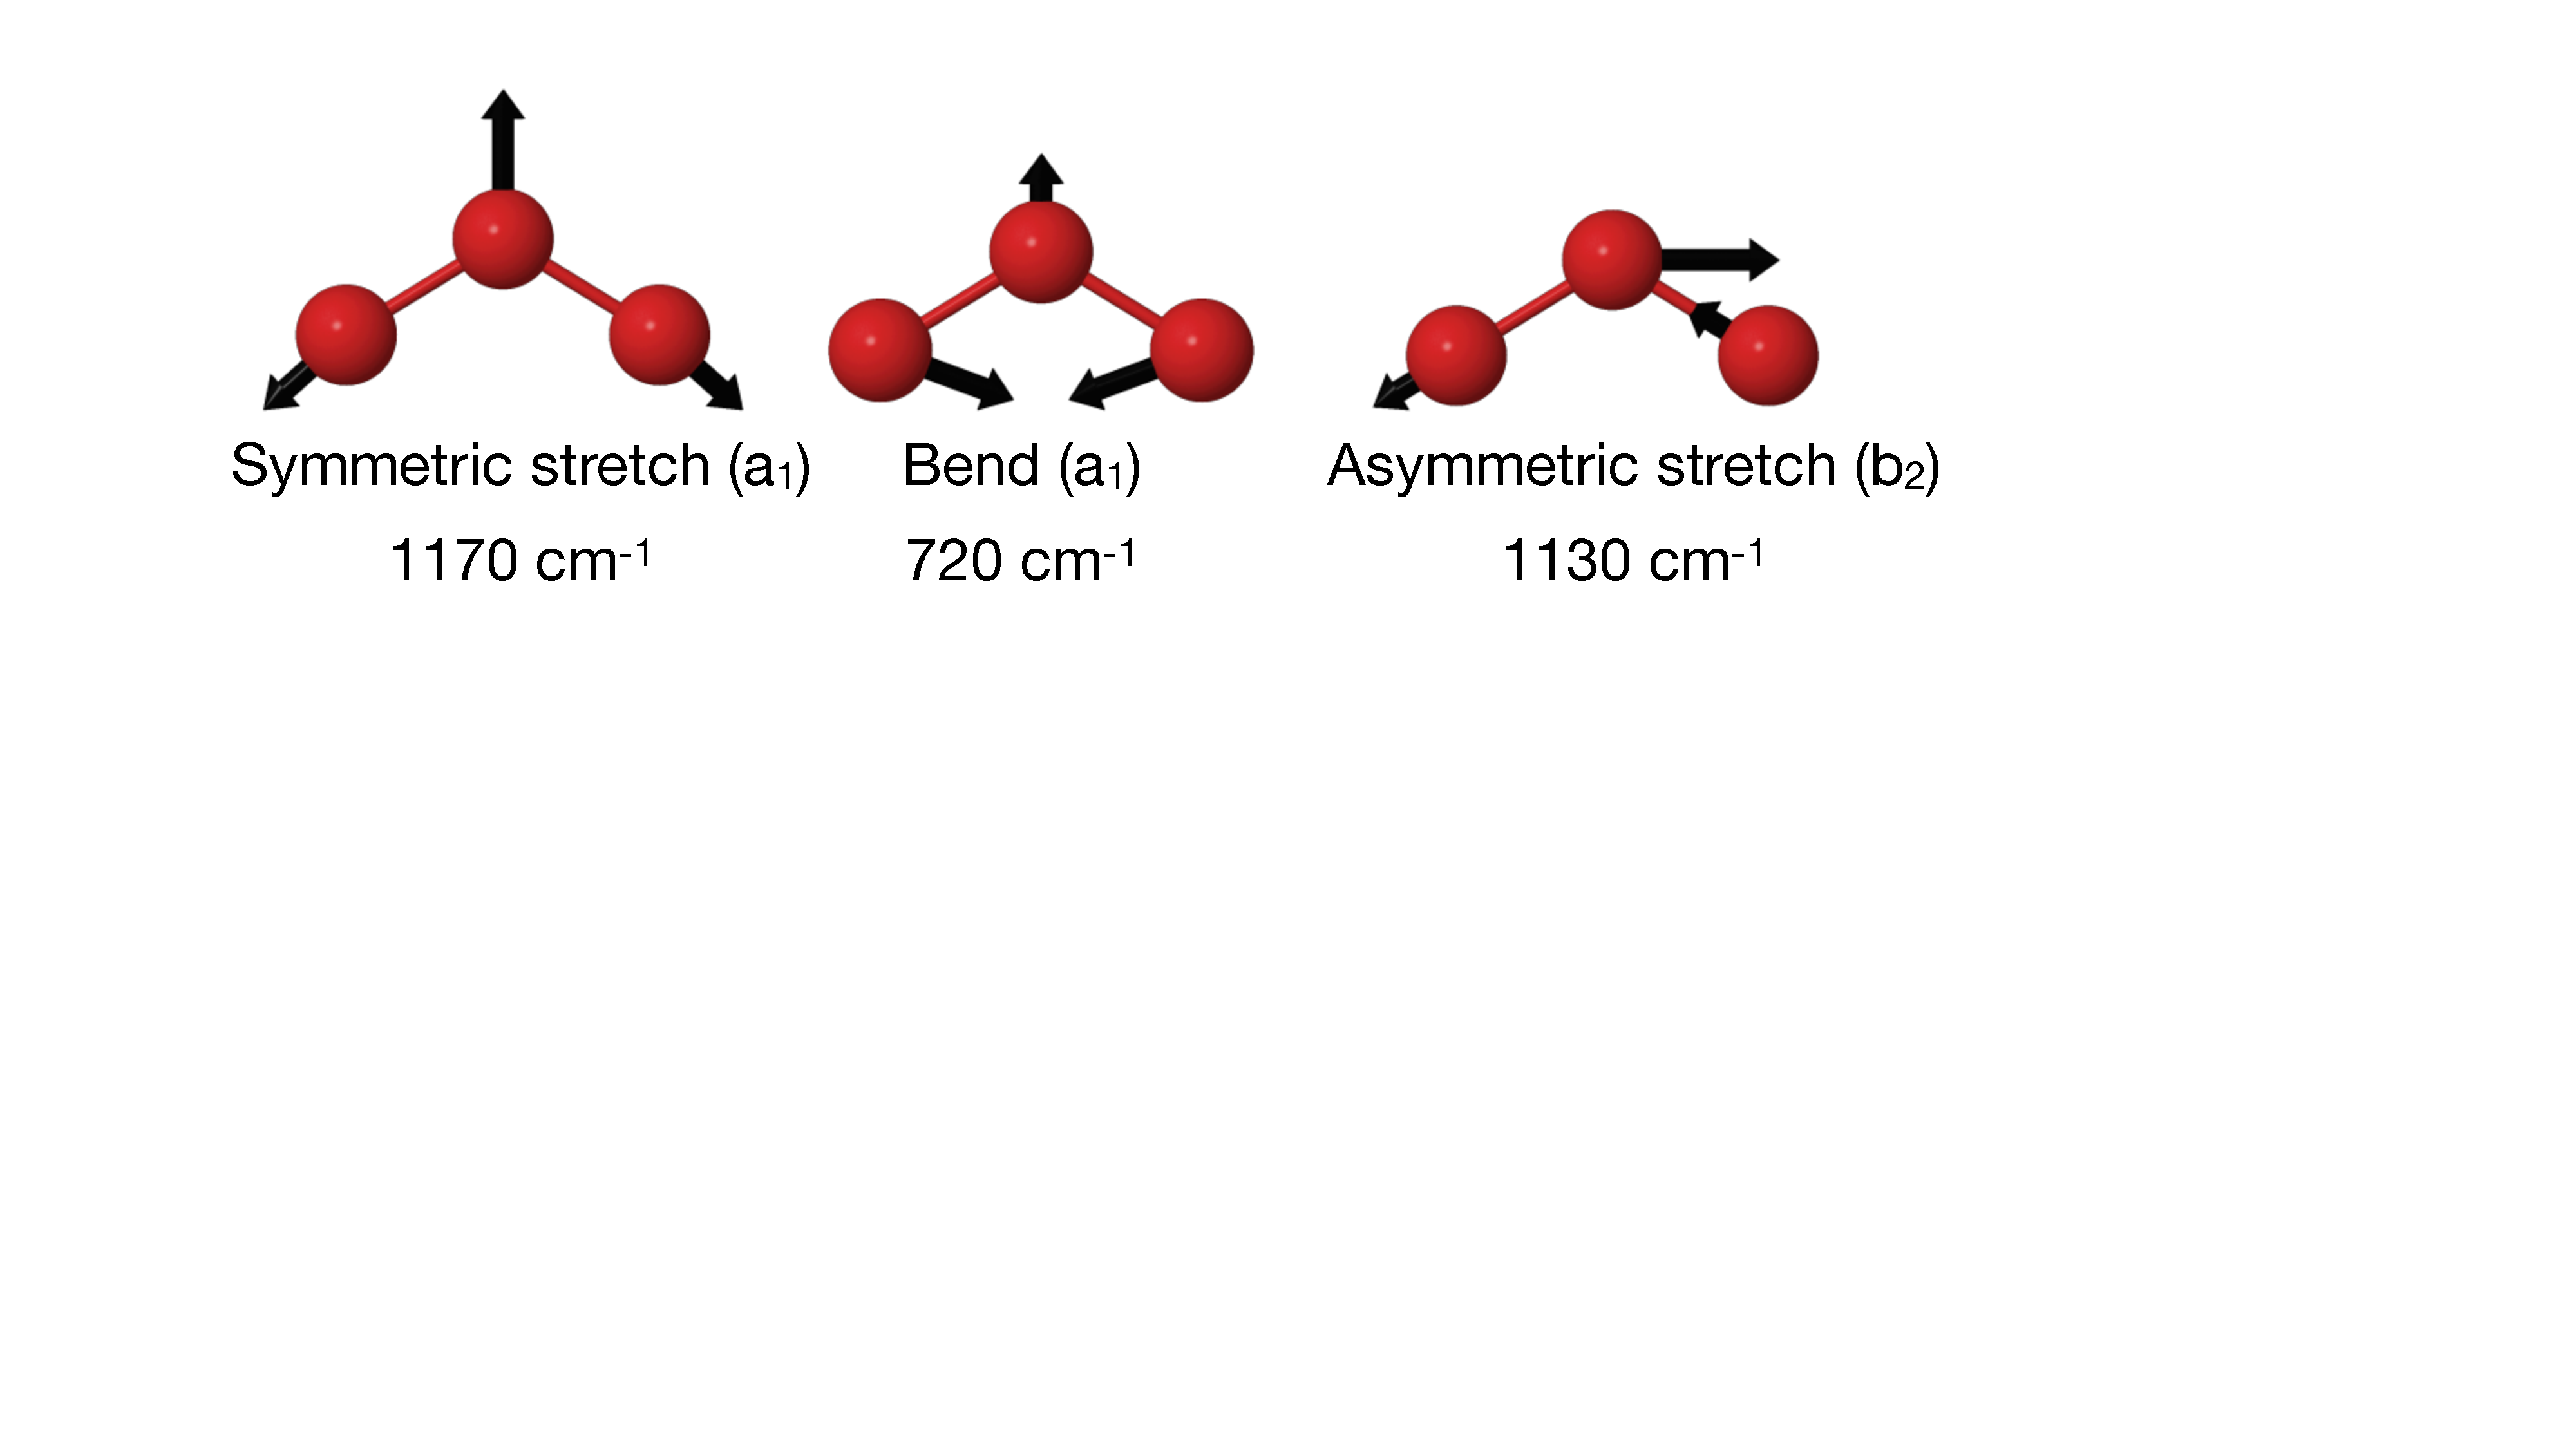
\includegraphics[width = 8 cm]{./figures/vibrations.pdf}
\caption{Three normal modes of the neutral ozone CCSDT/ANO1. Asymmetric stretching vibration of b$_2$ symmetry can couple the two lowest states of the cation ($^2$A$_1$ and $^2$B$_2$). 
\label{fig:vib}}
\end{figure}

The photoelectron spectrum of ozone has been reported\cite{dyke:O3:74} in 1974. Later,  much higher resolution of the positions of vibronic peaks was obtained with 
pulsed-field-ionization zero-kinetic-energy (PFI-ZEKE) spectroscopy \cite{Willitsch:O3ZEKE:2005}. From the theory side, the vibronic photoelectron spectrum of ozone was modeled with a vibronic Hamiltonian parameterized using multi-reference configuration interaction method
by Tarroni and Carter\cite{Willitsch:O3ZEKE:2005}.

Our contribution to this issue paying homage to the career and accomplishments
of R.J. Bartlett consists of an application of a vibronic coupling model,
parametrized by EOM-CC calculations, to the photoelectron spectrum of ozone.
We trust that this combination of methodology applied to a molecule that has
been extensively studied by the Bartlett group is an appropriate contribution.


%\begin{figure}
%    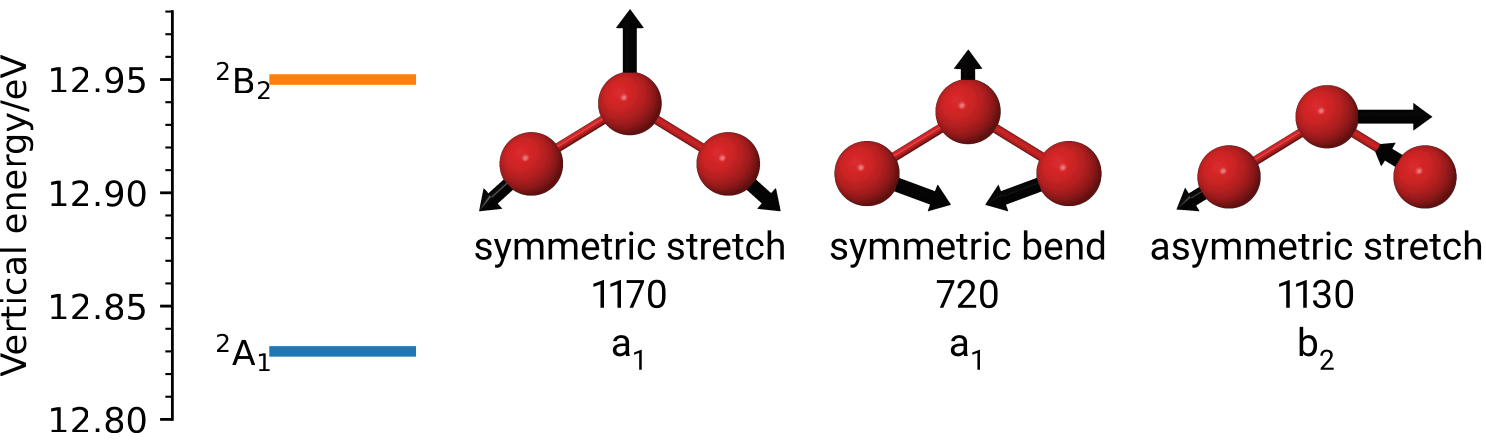
\includegraphics[width = 16 cm]{./figures/ozone_intro}
%    \caption{ 
%        Two lowest states of the ozone cation and normal modes of the ozone neutral.
%    }
%    \label{fig:ozone_intro}
%\end{figure}

\section{Theoretical models and computational details}

Ozone is a $C_{2v}$ molecule (following Mulliken's
convention~\cite{Mulliken:55:symnot}, the molecule is placed in the $yz$-plane
and the molecular symmetry axis aligns with the $z$-direction) with three
normal modes: symmetric stretch, symmetric bend, and asymmetric stretch (Fig. \ref{fig:vib}).  
The asymmetric stretch is of $b_2$ symmetry. The two lowest electronic states of
the ozone cation, $^2$A$_1$ and $^2$B$_2$, are very close in energy---separated by the gap 
of mere 0.123 eV (or 990 cm$^{-1}$)---and can be coupled by the b$_2$ vibration, giving rise
to significant vibronic effects in the photoelectron spectrum.  

We simulate the vibronic states of the ozone cation using the model
Hamiltonian of K{\"o}ppel, Domcke, and Cederbaum---the KDC
Hamiltonian\cite{Cederbaum:LVC:84,KDC:81,Koppel:CIbookCh7:04}. This is a
multi-state and multi-mode Hamiltonian defined in the basis of diabatic
states. For the ozone cation, the basis comprises two quasi-diabatic
states (related to the $^2$A$_1$ and $^2$B$_2$ states at the ground-state minimum), coupled by one mode (asymmetric 
stretch, mode number 3). 
The model also includes two symmetric modes (modes number 1 and 2). 
The matrix elements of the vibronic Hamiltonian are expanded around the equilibrium geometry
of neutral ozone using the respective dimensionless normal coordinates, 
$Q_i$, and the corresponding harmonic frequencies, $\omega_i$.
The overall form  of the vibronic Hamiltonian is thus: 
\begin{subequations}
    \begin{equation}
        H = H _0 \mathbf{1} +
        \begin{pmatrix}
            V^{(1)}  & \lambda _3 Q _3\\
            \lambda _3 Q _3 & V^{(2)}
        \end{pmatrix},
\end{equation}
where $H _0$ contains kinetic energy operator 
and a potential energy term for the coupling mode 
    \begin{equation}
        H _0 = 
        \frac{1}{2} \left(\sum _{i = 1}^3 
        - \omega _i \frac{\partial ^2}{\partial Q _i ^2 }\right)
        + \frac{1}{2}\omega _3 Q _3 ^2,
\end{equation}
and  $V^{(1)}$ and $V^{(1)}$ describe the two diabatic states expanded over $Q_1$ and $Q_2$
\begin{equation}
        V ^{(\alpha)} = 
        E ^{(\alpha)} 
        + \sum _{i \in \{1,2\}} 
            \kappa ^{(\alpha)} _i Q _i 
        + \sum _{i,j \in \{1,2\}} 
            \kappa ^{(\alpha)} _{ij} Q _i Q _j 
        + \sum _{i,j,k \in \{1,2\}} 
            \kappa ^{(\alpha)} _{ijk} Q _i Q _j Q _k 
        + \sum _{i,j,k,l \in \{1,2\}} 
            \kappa ^{(\alpha)} _{ijkl} Q_i Q _j Q _k Q _l.
    \end{equation}
    \label{eq:KDC}
\end{subequations}
Here $E ^{(\alpha)}$ are the vertical ionization energies
calculated at the equilibrium geometry of the neutral, $\kappa$ are the coefficients of expansion of the potential along the fully symmetric coordinates, 
and $\lambda$ is the linear diabatic coupling.
Fig. \ref{fig:KDC} shows the resulting diabatic potential energy surfaces. 
The displacements along the two symmetric normal modes are clearly visible, 
suggesting vibrational progressions along the bend and symmetric stretch.  

\begin{figure}[h!]
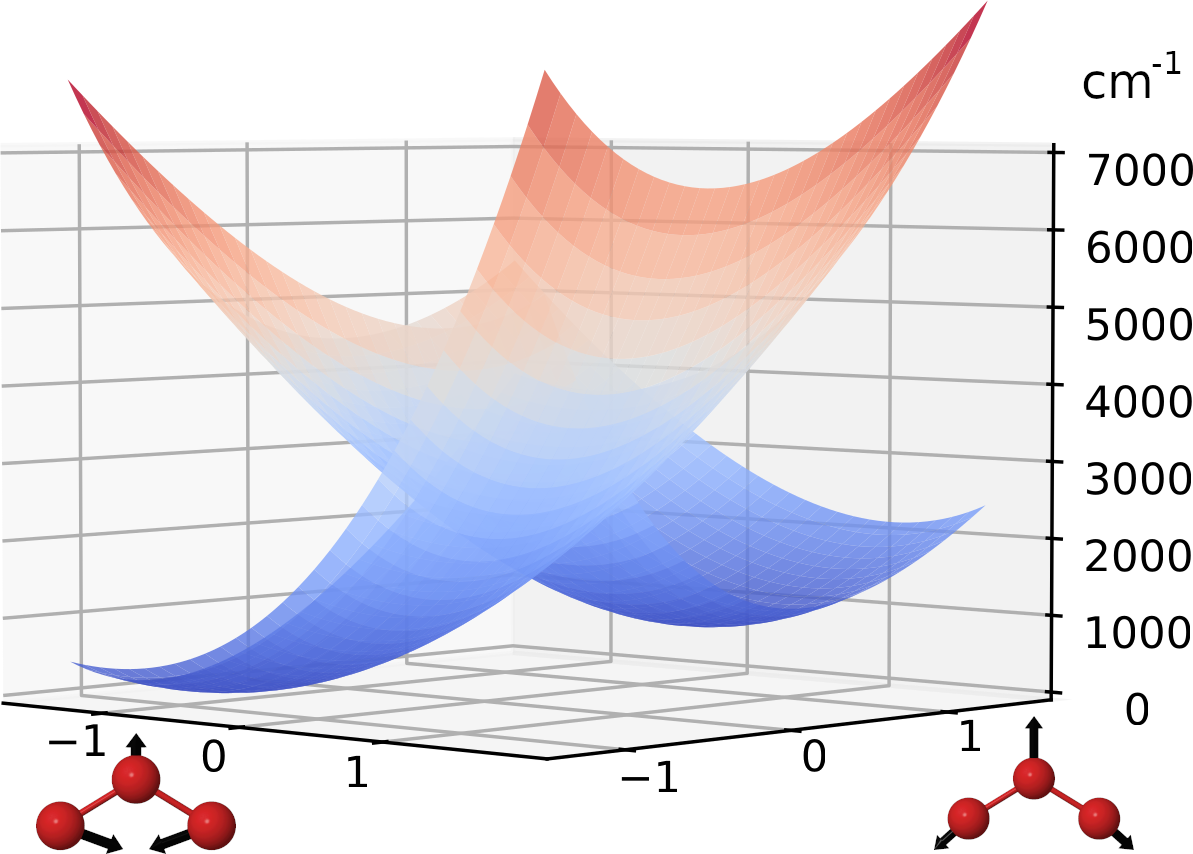
\includegraphics[width = 8 cm]{./figures/KDC_PES.png}
\caption{Cuts of potential energy surfaces of the two diabatic states of ozone cation 
(corresponding to the $^2$A$_1$ and $^2$B$_2$ states at the equilibrium geometry of the 
neutral) shown as function of the two stretching modes, $Q_1$ and $Q_2$, at $Q_3$=0.
%The displacements along the two symmetric normal modes are clearly visible. 
% Mode labels are correct
%Energy scale is in wavenumbers.
\label{fig:KDC}}
\end{figure}

We computed the parameters of the KDC Hamiltonian using \emph{ab
initio} CC and EOM-CC methods.~\cite{Bartlett:CC_review:07, Krylov:EOMRev:07, Bartlett:Book:09,Christiansen:EOMRev:11, Bartlet:EOMRev:12, Krylov:OSRev} 
We considered methods in which the CC expansion was truncated to singles and doubles (CCSD), singles, doubles and triples (CCSDT), as well as singles, doubles, triples and quadruples (CCSDTQ).\cite{Matthews:ncc:2015}  
We computed the geometry of the neutral ozone and its harmonic
frequencies and normal coordinates with CCSDT/ANO1.~\cite{Almlof:ANO,Almlof:ANO:1988} 

The optimized geometry of ozone has a bond length of 1.270 \AA\ and a
bond angle of 116.9$^\circ$. The two symmetric normal modes have frequencies
1,169~cm$^{-1}$ and 724~cm$^{-1}$, and the asymmetric stretch has a
frequency of 1,129~cm$^{-1}$. 

We described the states of the cation using 
EOM-CC for ionization energies (known as EOM-IP-CC).~\cite{StantonGauss:EOMIP:99} 
We used the definition of quasi-diabatic states by Ichino, Gauss, and Stanton\cite{Stanton:EOMIPdeg:09}  based on the  EOM-IP-CC method (EOMIP-CC-QD). 
We computed the linear diabatic coupling $\lambda$ and the expansion coefficients $\kappa$ at the equilibrium geometry of the neutral; $\lambda$ was computed with 
EOM-IP-CCSD-QD/ANO1 and  $\kappa$'s were computed using the
EOM-IP-CCSD/ANO1 energies calculated on a grid. The computed value of the linear diabatic coupling constant $\lambda$ is 1,394~cm$^{-1}$. The complete set of KDC parameters is given in the SI.


We computed the vertical ionization energies using a composite method.  The
starting value is the complete basis set (CBS) extrapolation of the
EOM-IP-CCSDT/cc-pCVnZ energies with n = 5, 6.~\cite{Woon:95:CCBS} These values
were augmented with two corrections: the $\Delta$Q correction in the cc-pwCVTZ
basis set and the relativistic correction calculated using
EOM-IP-CCSD/cc-pwCVTZ.~\cite{Dunning:02:p(w)CVnZ} 
The error bars were estimated as follows: 
for the extrapolated CBS reference values, we used half of the absolute value
of the difference between the best \emph{ab initio} value and the extrapolated
value, and for the remaining corrections (quadruples correction, $\Delta Q$, and
the relativistic correction) we used half of the
absolute value of the correction.

To compare the simulated photoelectron spectrum to the experimental one, 
we used the
cross-section ratio A$_1$:B$_2$ of $1$:$1.35$.\cite{KDC:O3:92}
Additionally, the stick spectrum was broadened with the Lorenzian envelopes
normalized to the feature intensities
\begin{equation}
    f(x, x _i, I _i) = 
    \frac{I_i}{(x-x _i)^2 + (\gamma/ 2) ^2},
    \label{eq:lorentzian}
\end{equation}
where $x_i$ is the position of the spectral peak, $I_i$ is its intensity and
$\gamma$ is the peak's width.


The spectrum was computed using the \textsc{xsim} module in \textsc{CFOUR},
with the basis of 50 harmonic states in each mode and 6,000 iterations of the
Lanczos procedure.~\cite{Sharma:xsim_socjt:2024} All electrons were correlated in all CC/EOM-CC calculations. All calculations were performed 
using \textsc{CFOUR}.~\cite{cfour, cfour:2020}

\section{Results and Discussion}

We begin by discussing the accuracy of the computed electronic states.
The vertical ionization energy for the first excited state, $E^{(1)}$, 
computed using the composite
method described above, is  12.827~eV. Our error estimate for this value is
30~meV (see Table~\ref{tab:vertical_ionization_energy} for details).  We note
that the convergence of the vertical gap between the two states is much faster
and this value is estimated as 123$\pm8$~meV (see Table~\ref{tab:vertical_gap}
for details). 

\begin{table}[h!]
\caption{
Vertical ionization energies with the error estimates, eV.
    \label{tab:vertical_ionization_energy}}
    \begin{center}  
        \begin{tabular}[c]{|l|rr|r|}
            \hline
            Contribution  & $^2$A$_1$ & $^2$B$_2$ & Error estimate \\ \hline
            EOM-CCSDT/CBS & 12.872    & 12.981    & 0.02 \\
            $\Delta$Q/pwCVTZ & -0.037    & -0.021    & 0.02 \\
            Relativistic/CCSD/pwCVTZ  & -0.008    & -0.010    & 0.005 \\ \hline
            Final value, eV           & 12.827    & 12.950    & 0.03 \\ \hline
        \end{tabular}
    \end{center}
\end{table}

\begin{table}[h!]
    \caption{
        The vertical energy gap between the $^2$A$_1$
        and $^2$B$_2$ states with error estimates, meV. 
        %See caption of Table~\ref{tab:vertical_ionization_energy}.
    \label{tab:vertical_gap}}
    \begin{center}
        \begin{tabular}[c]{|l|r|r|}
            \hline
            Contribution             &  Vertical gap    & Error estimate \\ \hline
            EOM-CCSDT/CBS            &  108.8           & 0.9 \\
            $\Delta$Q/pwCVTZ         &   16.5           & 8 \\
            Relativistic/CCSD/pwCVTZ &   -2.2           & 1.1 \\ \hline
            Final value, meV         &  123             & 8 \\
            Final value, cm$^{-1}$   &  990             & 65 \\ \hline
        \end{tabular}
    \end{center}
\end{table}


\begin{figure}
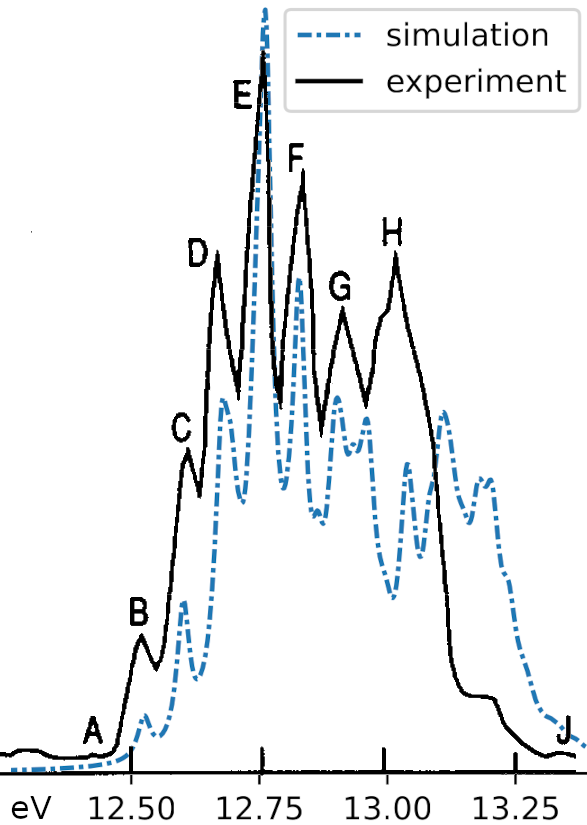
\includegraphics[width = 8 cm]{figures/sim_vs_Dyke.png}
\caption{
    Comparison of the experimental (solid black line digitized from Ref.~\citenum{dyke:O3:74}) and the simulated
    photoelectron spectra shown as electron binding energies.
    The simulated spectrum is blue-shifted by 21~meV and the peaks were broadened using  $\gamma$ = 30~meV.
    Used with permission of Royal Society of Chemistry, from Ref.~\citenum{dyke:O3:74} permission conveyed through Copyright Clearance Center, Inc.
\label{fig:sim_vs_dyke}}
\end{figure}


Figure~\ref{fig:sim_vs_dyke} compares the simulated spectrum to the
lower-resolution experimental spectrum taken from Ref.~\citenum{dyke:O3:74}. 
Peak A is
known to be a hot band, and does not appear in our (0~K)
simulation.~\cite{KDC:O3:92} The simulation reproduces well the consecutive
increase in the intensities of peaks B, C, D, and E as well as the spacing between these peaks. The drop in the intensity at peak F is
captured by the simulation. Starting from peak G, the simulation shows
discrepancy with the experiment. A sudden drop in the intensity past peak
H is not observed in the simulation. We discuss a likely source of this mismatch below.

Our simulation allows
for an additional element of analysis---Figure~\ref{fig:ozone_overlay} shows a decomposition of the simulated spectrum from Figure~\ref{fig:sim_vs_dyke}. 
All lines that contribute to the
spectrum are marked individually and are color-coded indicating which
electronic state's transition intensity the peak draws from. The total
envelope of the spectrum is also decomposed showing contributions from both
states. Our simulation locates the minimum of the conical intersection (marked as CI) at 3,174~cm$^{-1}$ above the origin (12.92~eV). 



\begin{figure}[h!]
%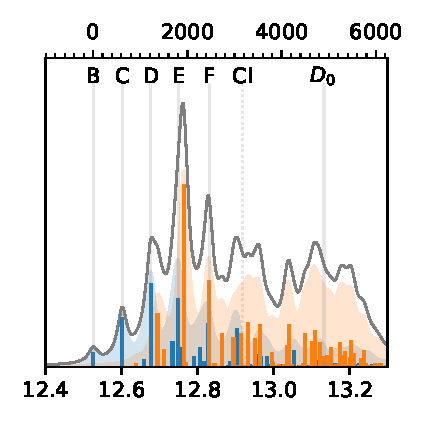
\includegraphics[width=8cm]{figures/spectrum_overline.pdf}
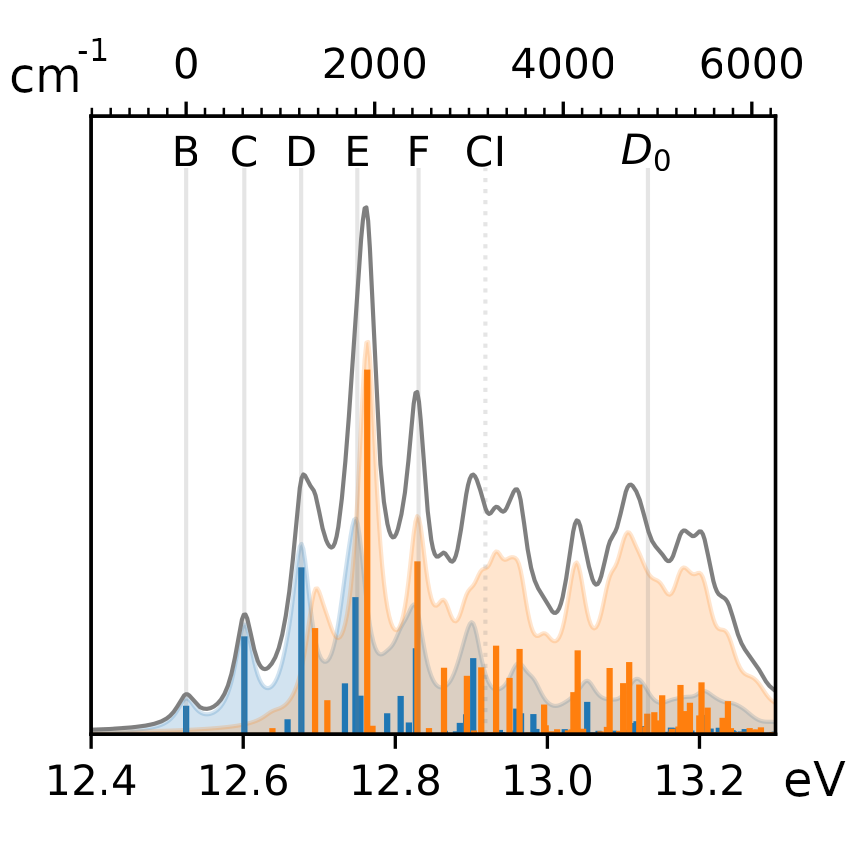
\includegraphics[width=8cm]{figures/spectrum_overline.png}
\caption{
        Simulated photoelectron spectrum of ozone shown as electron binding energies. Bottom axis shows energy
        scale in eV.  
        Top axis shows energy offset from the origin in
        cm$^{-1}$. 
        Stick spectrum shows positions and intensities of all
        simulated states. Blue and orange colors mark states of A$_1$ and
        B$_2$ symmetry, respectively. Gray vertical lines with captions on top
        indicate positions of features measured by the PFI-ZEKE
        experiment.~\cite{Willitsch:O3ZEKE:2005} The simulated spectrum was
        shifted to match the PFI-ZEKE experimental origin by 21~meV. 
        $D_0$ marks the dissociation threshold of O$_3^+$.~\cite{Willitsch:O3ZEKE:2005}
        Gray dotted line marks the energy of the minimum of the conical
        intersection (CI) as located by our Hamiltonian.
    \label{fig:ozone_overlay}}
\end{figure}

\begin{figure}[h!]
    % 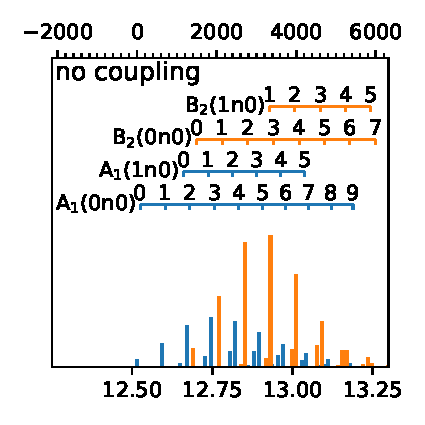
\includegraphics[width=10cm]{figures/spectrum_assigned.pdf}
    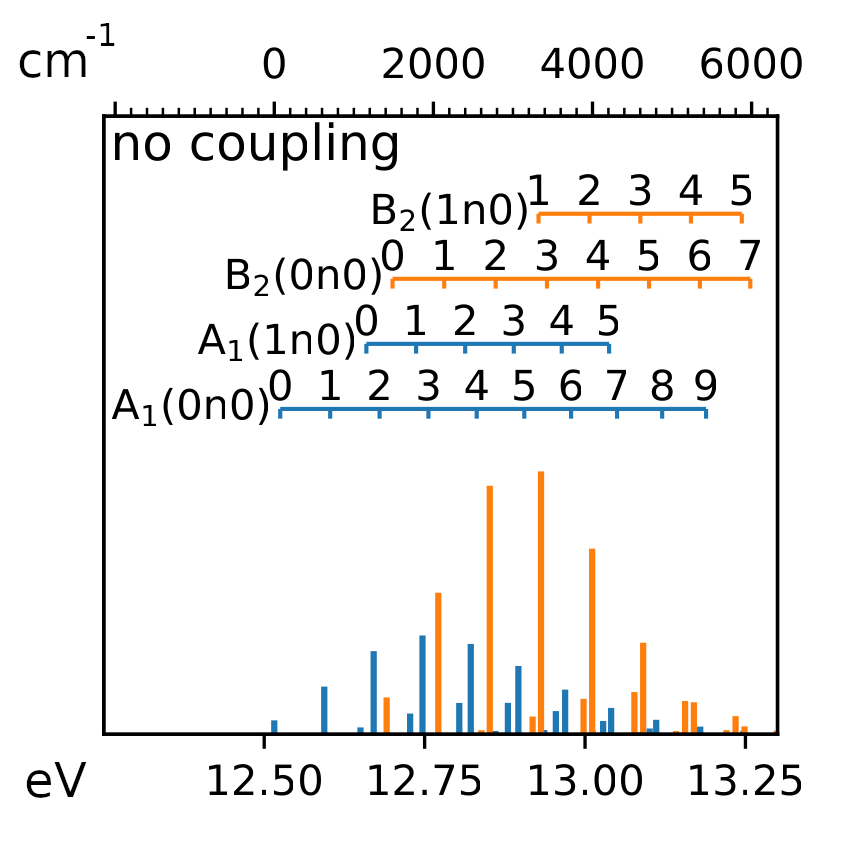
\includegraphics[width=10cm]{figures/spectrum_assigned.png}
    \caption{Simulated Franck-Condon photoelectron spectrum of ozone with vibronic
        coupling removed.
    \label{fig:no_coupling}}
\end{figure}

We assigned the vibronic peaks using a comparison to the Franck-Condon
simulation. To this end, the spectrum is simulated once again, this time,
however, setting the linear diabatic constant to zero ($\lambda$= 0).
This yields the spectra of the two electronic states 
at an equivalent level of theory but without vibronic coupling, i.e., the
combined Franck-Condon spectra of the two states.  
Figure~\ref{fig:no_coupling} shows this spectrum.
The non-coupled spectrum is easy to assign using the labels that mark the
symmetry of the electronic state, A$_1$ or B$_2$, and the vibrational state
($\nu _1 \nu_2 \nu_3$), where $\nu _i$ is the number of quanta in mode $i$
($i=1$ for the symmetric stretch, $i=2$ for the symmetric bend and $i=3$
for the asymmetric stretch). The assigned spectrum shows progressions in the
symmetric bend. There is one such progression in each electronic state.
Additionally for each state, there is also another progression in the
symmetric bend with one excitation in the symmetric stretch.

The decomposition of the spectrum presented on Figure~\ref{fig:ozone_overlay}
provides additional insight. The spectrum shows that peaks B and C are
almost purely of the $^2$A$_1$ electronic and $a_1$ vibrational character.
Starting from the peak D, the contributions from two states are of equal
magnitude. It is also clear that the following peaks comprise mixtures of many
vibronic peaks. At the energy of about 2,000~cm$^{-1}$ above the origin the
density of vibronic peaks increases significantly. This value can be compared
to the minimum of the conical intersection located at about 1,000~cm$^{-1}$
above the origin. Our Hamiltonian  is not suitable for describing dissociation of the
molecule, therefore, we expect a discrepancy with the experiment as the energy
gets closer to the dissociation threshold located at 4,898$\pm$3~cm$^{-1}$
above the origin.~\cite{Willitsch:O3ZEKE:2005}

\begin{figure}[h!]
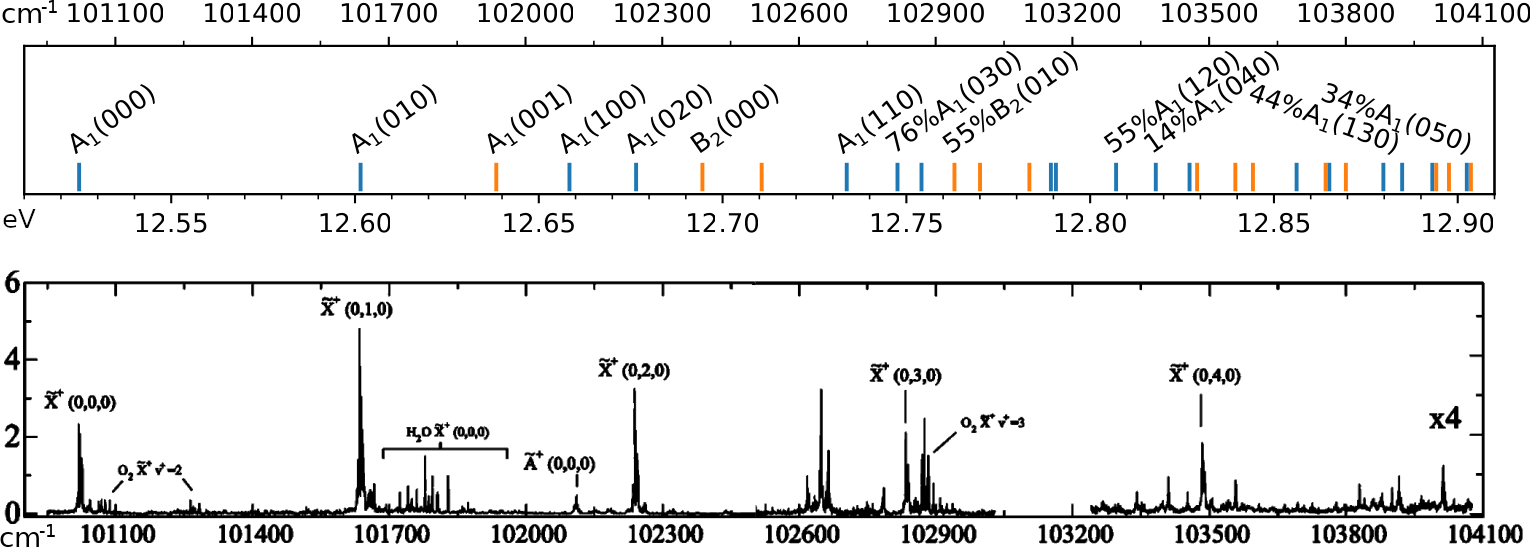
\includegraphics[width=16 cm]{./figures/sim_vs_zeke.png}
\caption{
        Comparison of the simulated spectrum with the PFI-ZEKE
        experiment.\cite{Willitsch:O3ZEKE:2005} The simulated spectrum was
        blue-shifted by 21~meV = 170~cm$^{-1}$. The bottom panel is adapted from 
        Ref. \citenum{Willitsch:O3ZEKE:2005}.
        The bottom panel adapted with permission from Ref. \citenum{Willitsch:O3ZEKE:2005} copyright AIP Publishing LLC.
    \label{fig:sim_vs_zeke}}
\end{figure}

%The vibronic states are decomposed in the basis of the artificial, uncoupled states discussed in the previous paragraph.  
Figure~\ref{fig:sim_vs_zeke}
shows the assigned spectrum and Table~\ref{tab:peak_assignment} lists the
decomposition of all peaks in the region of up to 3100~cm$^{-1}$. 
We compare the resulting assignment with the high-resolution
PFI-ZEKE spectrum from
Ref.~\citenum{Willitsch:O3ZEKE:2005}. The PFI-ZEKE spectrum is the best source of
information on the location of the peaks, especially the origin, against which
the origin peak of the simulation is aligned. The origin of the simulated
spectrum is red-shifted by 170~cm$^{-1}$ relative to the experimental origin at 101,020.5~cm$^{-1}$.\cite{Willitsch:O3ZEKE:2005} This discrepancy is within
our error estimate for the vertical ionization energy
(30~meV=240~cm$^{-1}$).  

The comparison with the high-resolution spectrum (Fig.~\ref{fig:sim_vs_zeke}) reveals more details. Lines of the PFI-ZEKE
experiment and our simulation match very well. Especially the states of the
A$_1$ symmetry are well aligned with the experimental features. States close
to the origin are similar to the non-coupled states. The origin peak is of
A$_1$(0,0,0) character, the first two excitations in the symmetric bend,
A$_1$(0,1,0) and A$_1$(0,2,0) are also very similar to the non-coupled states,
whereas the higher excitations in this progression show significant mixing. The
same progression with one vibrational quanta in the symmetric stretch is more
interesting. The first of its peaks is very well aligned with experimentally
visible feature, which was previously assigned as the origin of the second
electronic state. The second peak in this series, A$_1$(1,1,0), has very high
similarity to its uncoupled version. It is a good candidate to assign the
experimental, unassigned feature above 102,600~cm$^{-1}$.

States of the B$_2$ symmetry, on the other hand, do not align well with
the experiment. The first such peak, close to the 12.64~eV mark in
Figure~\ref{fig:sim_vs_zeke}, is assigned to the A$_1$(0,0,1) state.  This is
a vibronic state that gains intensity owing to the coupling to the electronic
$^2$B$_2$ state. This vibronic peak lies in the part of the spectrum where
bands of oxygen (which appears as impurity in the gas sample) are visible in
the experiment. The origin of the $^2$B$_2$ state is very similar to the
uncoupled B$_2$(0,0,0) state, but it is located in an empty area of the
experimental spectrum. The next peak, slightly above a 12.76~eV mark in
Figure~\ref{fig:sim_vs_zeke}, corresponds to the one excitation of the
symmetric bend in the $^2$B$_2$ state, but as the label on the figure shows,
it is only about 55\% similar to the uncoupled state.

\begin{figure}
    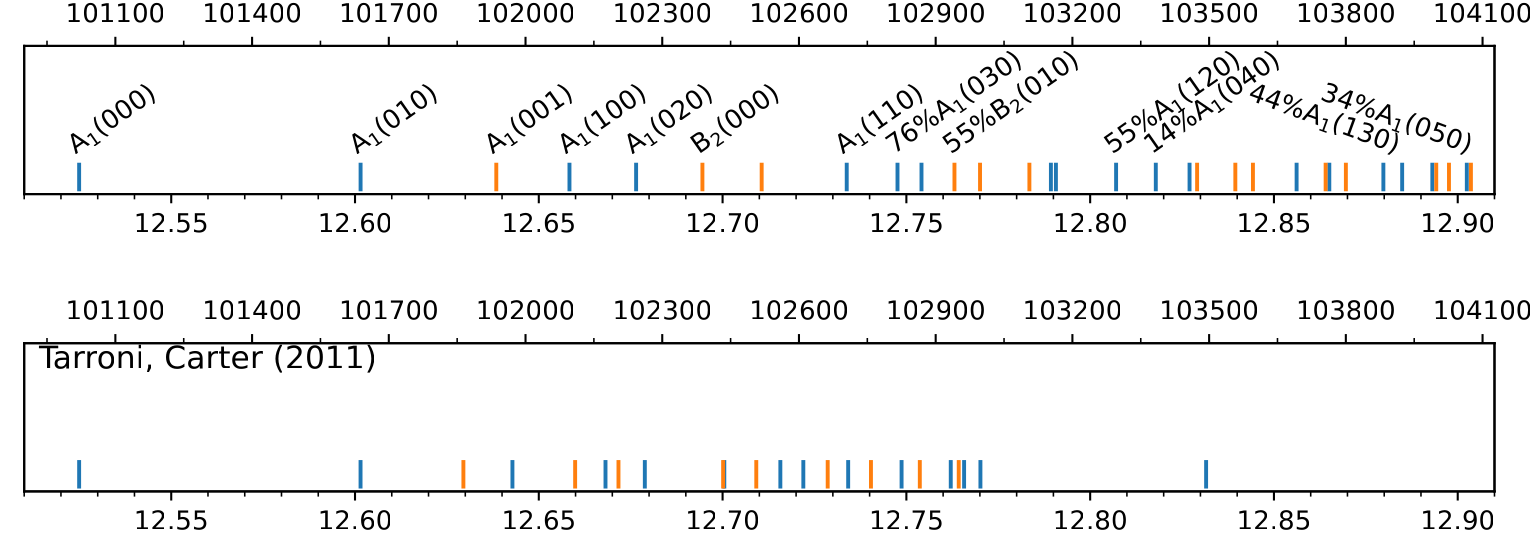
\includegraphics[width=16 cm]{figures/sim_vs_TarroniCarter.png}
    \caption{Comparison of the simulated spectrum to an earlier simulation
        by Tarroni and Carter (assigned lines).~\cite{tarroni:O3:2011}
    \label{fig:sim_vs_tarronicarter}}
\end{figure}

Finally, Figure~\ref{fig:sim_vs_tarronicarter} compares our spectrum to
an earlier accurate simulation using multi-reference configuration interaction 
by Tarroni and Carter\cite{Willitsch:O3ZEKE:2005}. The comparison includes only the lines
from the earlier simulation that were tabulated with an assignment. 
The comparison to the earlier simulation in
Figure~\ref{fig:sim_vs_tarronicarter} shows that both match well with
the experiment. Both simulations also agree in the assignment of the first
progression in the bending mode. The previous simulation, however, shows
smaller spacing between the remaining lines, yielding much higher congestion of
the spectrum. Additionally, the origin of the second state falls at lower
energy aligns well with the peak that was assigned in the PFI-ZEKE
experiment also as the origin of the second state. While an additional
simulation of the line intensities would allow for the most complete
comparison to the experimental spectrum, the strong alignment of the simulated
peaks of a A$_1$ symmetry with the experimental features leads us to
believe that our simulation offers the best assignment of the spectrum to
date.

\begin{table}[h!]
\renewcommand{\arraystretch}{0.8}% Tighter
\caption{Assignment and decomposition of the eigenvectors of the ozone
    cation. The first column shows the offset of simulated peaks from 
    the origin in cm$^{-1}$.
    \label{tab:peak_assignment}}
    \begin{tabular}{|l|l|l|l|}
        \hline
        Offset & Symmetry& Assignment & Eigenvector \\
        \hline
$     0$ & $A_1$ &  $A_1(000)$ & $ +0.99~A_1(000)$ \\
$   618$ & $A_1$ &  $A_1(010)$ & $ +0.99~A_1(010)$ \\
$   915$ & $B_2$ &  $A_1(001)$ & \\
$  1076$ & $A_1$ &  $A_1(100)$ & $ -0.99~A_1(100)$ \\
$  1222$ & $A_1$ &  $A_1(020)$ & $ +0.97~A_1(020)$ \\
$  1368$ & $B_2$ &  $B_2(000)$ & $ +0.97~B_2(000)$ \\
$  1498$ & $B_2$ &             & $ +0.10~B_2(000)$ \\
$  1684$ & $A_1$ &  $A_1(110)$ & $ +0.96~A_1(110)$ \\
$  1796$ & $A_1$ &  $A_1(030)$ & $ +0.87~A_1(030) +0.16~A_1(110) +0.13~A_1(020) -0.13~A_1(040)$ \\
$  1848$ & $A_1$ &             & $ -0.31~A_1(030)$ \\
$  1921$ & $B_2$ &  $B_2(010)$ & $ +0.74~B_2(010) -0.18~B_2(020) -0.11~B_2(000)$ \\
$  1977$ & $B_2$ &             & $ -0.24~B_2(010)$ \\
$  2085$ & $B_2$ &             & $ +0.52~B_2(010)$ \\
$  2132$ & $A_1$ &             & $ -0.25~A_1(030) -0.25~A_1(040) -0.13~A_1(120) +0.13~A_1(050)$ \\
$  2143$ & $A_1$ &             & \\
$  2275$ & $A_1$ &  $A_1(120)$ & $ +0.86~A_1(120) +0.12~A_1(040)$ \\
$  2362$ & $A_1$ &             & $ -0.62~A_1(040) +0.40~A_1(120) -0.17~A_1(030) +0.11~A_1(050)$ \\
$  2437$ & $A_1$ &             & $ -0.48~A_1(040) -0.11~A_1(120)$ \\
$  2453$ & $B_2$ &  $B_2(020)$ & $ +0.54~B_2(020) +0.25~B_2(010) -0.17~B_2(030)$ \\
$  2537$ & $B_2$ &             & \\
$  2576$ & $B_2$ &             & $ +0.27~B_2(020)$ \\
$  2671$ & $A_1$ &             & $ -0.48~A_1(040) -0.26~A_1(050) -0.19~A_1(130) -0.14~A_1(060)$ \\
$  2735$ & $B_2$ &             & $ +0.62~B_2(020)$ \\
$  2743$ & $A_1$ &             & \\
$  2780$ & $B_2$ &             & $ +0.22~B_2(020)$ \\
$  2862$ & $A_1$ &  $A_1(130)$ & $ +0.74~A_1(130) +0.13~A_1(120) -0.13~A_1(050)$ \\
$  2903$ & $A_1$ &             & $ -0.42~A_1(130)$ \\
$  2969$ & $A_1$ &             & $ -0.25~A_1(130) +0.17~A_1(050) +0.12~A_1(040)$ \\
$  2978$ & $B_2$ &             & $ -0.24~B_2(110) -0.19~B_2(020) +0.12~B_2(010)$ \\
$  3006$ & $B_2$ &             & $ -0.20~B_2(030) +0.17~B_2(110) -0.15~B_2(020)$ \\
$  3045$ & $A_1$ &  $A_1(050)$ & $ +0.79~A_1(050)$ \\
$  3054$ & $B_2$ &             & $ +0.29~B_2(110) -0.25~B_2(030) -0.13~B_2(020)$ \\
        \hline
    \end{tabular}
\end{table}

\section{Summary and Conclusions} 

In this exploration of the photoelectron spectrum of the ozone molecule,
we have deployed cutting-edge high-order CC models together with a
vibronic Hamiltonian approach to spectroscopy beyond the Born-Oppenheimer
approximation \cite{Cederbaum:LVC:84, KDC:81, Koppel:CIbookCh7:04}.
We parameterized the Hamiltonian using EOM-IP-CC calculations  and the formalism 
of quasi-diabatic states of Ichino, Gauss and Stanton.~\cite{Stanton:EOMIPdeg:09}
The results of the simulation are in excellent agreement with the experimental
spectrum from the ionization energy of the lower state to about 2,500
cm$^{-1}$ higher (the restriction arising from the local parametrization of
the Hamiltonian).  %{\bf confused, need to discuss}
Analysis of the spectrum and its simulation underscore the
importance of vibronic coupling effects in the ozone cation.  Results of this
work offer a state-of-the-art insight into the details of the spectrum and
allows for an assignment of the experimental results.  Simulated peaks that
gain intensity from the ${\tilde A}$B$_2$ state are absent in the PFI-ZEKE
spectrum which offers an interesting avenue for further investigations. 

\section{Acknowledgments} 

This project was initiated when three of the authors (P.W, P.G.S., and J.F.S)
were in Budapest, where J.F.S. was serving as a recipient of the John von
Neumann Award in STEM bestowed by the Fulbright Foundation. 
P.G.S. acknowledges support by National Research, Development and Innovation Fund (NKFIF) of Hungary (Grant No. 142634). Additional
research presented here benefited from the NSF Center for Chemical Innovation
Phase I (grant no. CHE-2221453) and the U.S. Department of Energy, Basic Energy
Sciences (grant no. DE-FG02-05ER15629).  The authors wish
Prof. Bartlett a happy ninth decade of life and hope that he continues to
stimulate others in the field with his creative insights.

\section*{Conflicts of interest}
The authors declare the following competing financial interest(s):
A.I.K. is the president and a part-owner of Q-Chem, Inc.

\section*{Data availability}
The data that support the findings of this study are available within the article and the associated SI.
\clearpage

\bibliographystyle{prf}
%Will remove ozone later, already in cvs
\bibliography{allrefs}


\end{document}
